% Results and discussion draft, 21 October 2026.
% Keep discussion_figures/ beside this source when copying to your report.
% All tables and figures belong to the revised notebook run, 21 October 2026.
% To incorporate into the main report, use the marked body and its figure folder.
\documentclass[a4paper,12pt]{article}
\usepackage[T1]{fontenc}
\usepackage[utf8]{inputenc}
\usepackage[margin=25mm]{geometry}
\usepackage{lmodern,microtype}
\usepackage{amsmath,graphicx}
\usepackage{array,booktabs,tabularx}
\usepackage{placeins}
\usepackage{xurl}
\usepackage[hidelinks]{hyperref}
\usepackage{caption}
\captionsetup{font=small,labelfont=bf}
\newcolumntype{Y}{>{\raggedright\arraybackslash}X}
\setlength{\parindent}{0pt}
\setlength{\parskip}{0.5em}
\setlength{\emergencystretch}{3em}
\renewcommand{\arraystretch}{1.15}
\renewcommand{\thefigure}{6.\arabic{figure}}
\renewcommand{\thetable}{6.\arabic{table}}
\graphicspath{{discussion_figures/}}
\hypersetup{pdftitle={Results and discussion working draft},pdfauthor={Yeshlen Moodley}}
\begin{document}
\setcounter{section}{5}
% BEGIN DISCUSSION BODY

\section{Results and discussion}

The evaluation examined whether behavioural risk scoring could identify suspicious cardless withdrawal vouchers while limiting alerts on legitimate activity. This chapter first considers the records produced by the simulator and the behaviour visible in the data. It then compares the scoring methods at voucher creation and cash-out, before examining missed scams and false alerts in more detail. These findings provide the basis for considering how the prototype could support the review of high-risk vouchers.

\FloatBarrier\subsection{Dataset checks and exploratory analysis}

The first part of the evaluation considered whether the simulator had produced usable records for the model comparison. Over the 180-day observation period, 19,078 active customers created 216,147 vouchers, of which 2,761 were labelled as scams. Scams therefore accounted for 1.28\% of the vouchers, leaving the scoring methods to identify a small minority within a much larger volume of legitimate activity. Most vouchers were redeemed, with 209,222 cash-outs recorded during the observation window.

Before examining differences between the classes, the records were checked against the product constraints and the information required for scoring. All 20 checks returned zero violations, including those covering amount increments, sending limits, redemption timing and consistency of customer history. There were also no duplicate voucher identifiers or disagreements between feature labels and the truth file. These results established that the records met the implemented checks, allowing the comparison to proceed without the identified forms of invalid or inconsistent data.

EDA then considered whether the behaviours used for scoring differed between legitimate and scam vouchers. To examine these patterns before evaluating the models, class comparisons used activity from the fitting and validation periods. Amount was one visible difference: scam vouchers had a median of R1,800, compared with R600 for legitimate vouchers. The difference remained when amounts were considered relative to the customer's preceding 90-day average, with median ratios of 1.68 and 1.00. This showed why customer history could provide useful context for the amount being sent, although the overlapping distributions meant that a large voucher could still be legitimate.

The time taken to redeem a voucher provided another view of the behaviour surrounding the transaction. As shown in Figure 6.1, 58.5\% of scam redemptions occurred within 15 minutes, compared with 9.1\% of legitimate redemptions. Rapid cash-out was therefore more common in the simulated scams, making it a relevant pattern to examine at the second scoring point. However, its presence in legitimate payments also showed why it could not establish fraud by itself.

\begin{figure}[htbp]
\centering
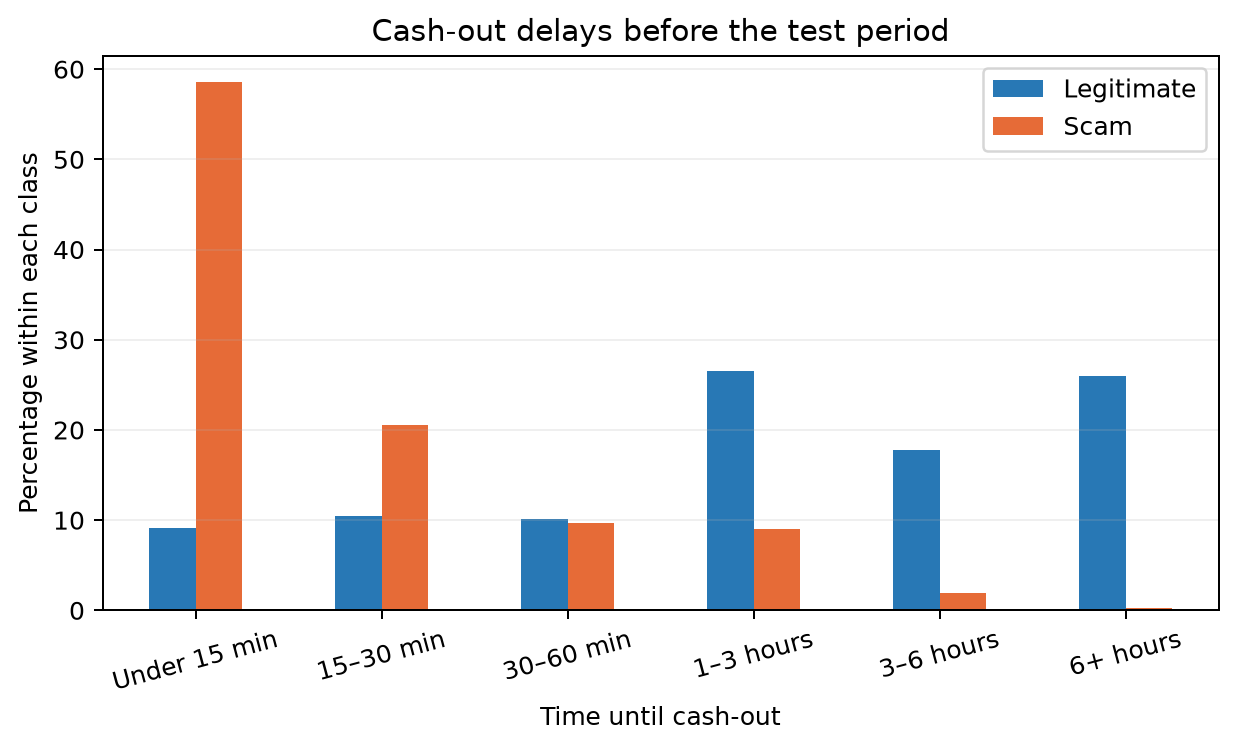
\includegraphics[width=.92\linewidth]{discussion_figures/eda_cashout_delays.png}
\caption{Cash-out delays as percentages within each class, using redemptions before the test boundary. The final range includes all delays of six hours or more.}
\end{figure}

A similar issue was visible in recipient and account changes. An unfamiliar recipient appeared in 68.6\% of scam vouchers, but also in 45.0\% of legitimate vouchers, so flagging every first-time recipient would affect many legitimate payments. Recent limit changes showed a clearer difference between the classes, occurring in 35.1\% of scam vouchers and 1.3\% of legitimate vouchers. Recent device changes were less frequent in both, at 5.8\% and 1.7\%, respectively. These patterns reflected the behaviour specified in the simulator and indicated where the classes differed; they did not measure the importance of each feature to a model.

Taken together, the EDA showed both differences and overlap in the simulated activity. The scoring methods had behavioural information to work with, but none of these individual observations made unusual activity equivalent to fraud. The next part of the evaluation therefore examined whether rules, anomaly models and their combination could distinguish the classes more effectively.

\FloatBarrier\subsection{Model results at creation and cash-out}

Rules provided the baseline for assessing whether anomaly detection added value to the warning indicators already defined in the prototype. Three anomaly models were compared with this baseline, and the strongest anomaly model on validation data was combined equally with rules. Validation selected One-Class SVM for this combination at both stages, using nu = 0.1, while LOF selected 100 neighbours. The following test results use these saved settings and validation-selected alert thresholds, allowing the comparison to assess decisions fixed before test scoring.

At voucher creation, the hybrid achieved the highest F1 of the five approaches, at 0.457, compared with 0.394 for rules alone (Table 6.1). This improvement came through higher recall: the hybrid detected 52.1\% of scam vouchers, compared with 31.9\% for rules. Its precision was lower, however, falling from 51.3\% for rules to 40.8\%. The hybrid therefore identified more scams at the cost of a larger proportion of false alerts. F1 summarises the balance between precision and recall, but both measures are needed to understand that trade-off (\href{https://fraud-detection-handbook.github.io/fraud-detection-handbook/Chapter\_4\_PerformanceMetrics/ThresholdBased.html}{Le Borgne et al., 2022}).

\begin{table}[htbp]
\centering\small
\caption{Test results at voucher creation. Hybrid means the equal blend of rules and One-Class SVM. FPR is reported as a percentage.}
\begin{tabularx}{\linewidth}{Yrrrr}
\toprule
\textbf{Approach} & \textbf{Precision} & \textbf{Recall} & \textbf{F1} & \textbf{FPR (\%)} \\
\midrule
Rules & 0.513 & 0.319 & 0.394 & 0.425 \\
Isolation Forest & 0.415 & 0.301 & 0.349 & 0.597 \\
LOF & 0.281 & 0.288 & 0.284 & 1.038 \\
One-Class SVM & 0.374 & 0.386 & 0.380 & 0.905 \\
Hybrid & 0.408 & 0.521 & 0.457 & 1.061 \\
\bottomrule
\end{tabularx}
\end{table}

None of the individual anomaly models exceeded the rule baseline's test F1 at creation. This was relevant to the purpose of the comparison: learning unusual patterns did not, on its own, produce a better balance of detection and false alerts than the explicit warning rules. The hybrid result nevertheless showed that combining anomaly information with those rules could improve that balance within the simulation. The benefit came from how the two components were used together, rather than from replacing the rules with an anomaly model.

At cash-out, the hybrid again achieved the highest F1, reaching 0.545, while rules reached 0.476 (Table 6.2). The same trade-off remained: rules had higher precision, at 63.9\%, while the hybrid detected a larger share of scams, with recall of 54.0\%. The preferred approach would therefore depend on whether the priority was to identify more scams or to limit the number of legitimate vouchers requiring review. Under the F1 measure used in this experiment, the hybrid provided the stronger combined result.

\begin{table}[htbp]
\centering\small
\caption{Test results at cash-out. Records enter this period according to cash-out time.}
\begin{tabularx}{\linewidth}{Yrrrr}
\toprule
\textbf{Approach} & \textbf{Precision} & \textbf{Recall} & \textbf{F1} & \textbf{FPR (\%)} \\
\midrule
Rules & 0.639 & 0.380 & 0.476 & 0.311 \\
Isolation Forest & 0.330 & 0.331 & 0.331 & 0.974 \\
LOF & 0.385 & 0.331 & 0.356 & 0.768 \\
One-Class SVM & 0.283 & 0.495 & 0.360 & 1.821 \\
Hybrid & 0.550 & 0.540 & 0.545 & 0.641 \\
\bottomrule
\end{tabularx}
\end{table}

The stage comparison in Figure 6.2 also shows that the cash-out results were not uniformly better for every method. Isolation Forest and One-Class SVM had lower F1 at cash-out, while rules, LOF and the hybrid had higher F1. For the hybrid, precision increased from 40.8\% at creation to 55.0\% at cash-out, whereas recall changed more modestly, from 52.1\% to 54.0\%. The main difference was therefore in how often its alerts were correct. However, Stage A evaluated 83,947 vouchers and Stage B evaluated 81,208, with periods assigned by their respective scoring times and thresholds selected separately. These results compare the two scoring stages; they do not isolate the effect of adding redemption features alone.

\begin{figure}[htbp]
\centering
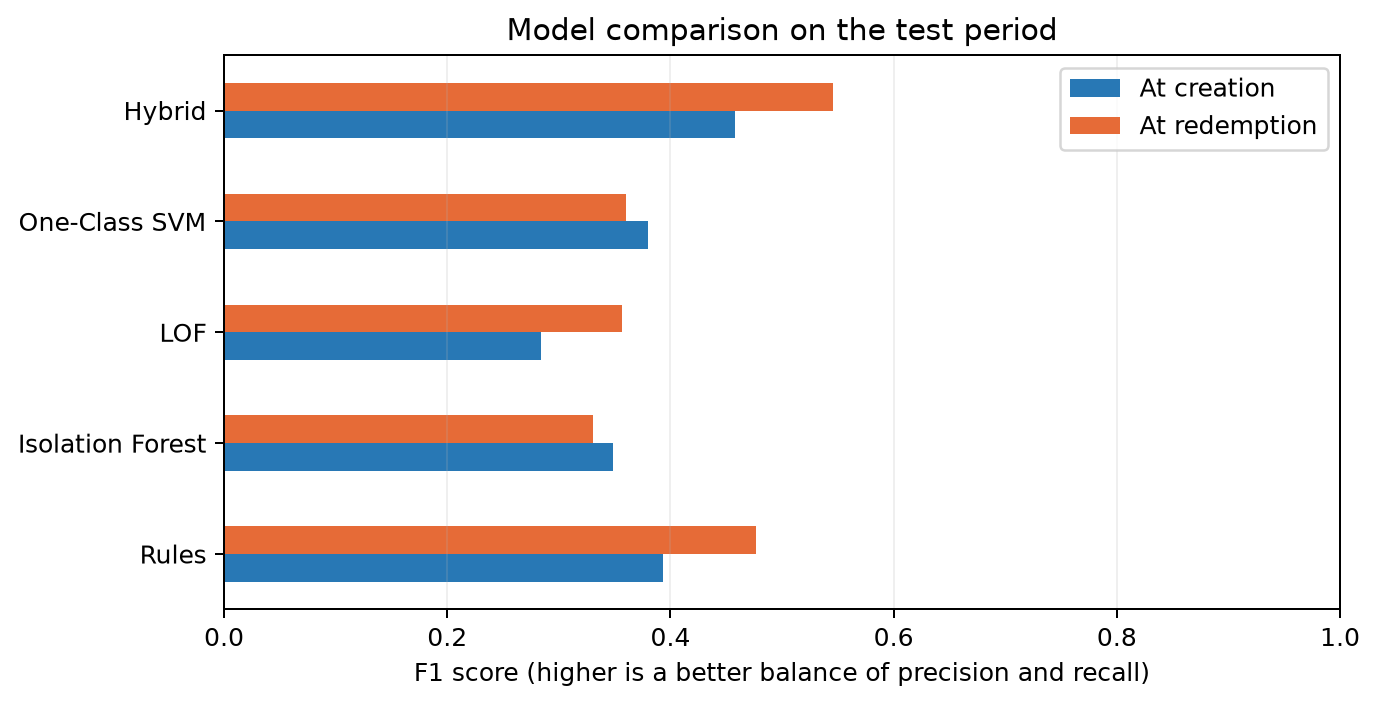
\includegraphics[width=.92\linewidth]{discussion_figures/model_f1.png}
\caption{Test F1 at creation and cash-out. Hybrid uses rules and One-Class SVM at both stages.}
\end{figure}

\FloatBarrier\subsection{Scams detected, missed scams and false alerts}

The metric comparison showed that the hybrid improved F1, but the decision counts help explain what this would mean for the vouchers being reviewed. At creation, the hybrid detected 605 scams and missed 557, while also flagging 878 legitimate vouchers (Table 6.3). Rules alone detected 371 scams and flagged 352 legitimate vouchers. The number of scams detected was therefore 234 higher with the hybrid, alongside 526 more legitimate vouchers flagged. Its increased detection would need to be considered together with this additional review burden.

\begin{table}[htbp]
\centering\small
\caption{Hybrid confusion-matrix counts on the test period.}
\begin{tabularx}{\linewidth}{Yrr}
\toprule
\textbf{Hybrid decision} & \textbf{Creation} & \textbf{Cash-out} \\
\midrule
Scams detected & 605 & 628 \\
Scams missed & 557 & 534 \\
Legitimate vouchers flagged & 878 & 513 \\
Legitimate vouchers left unflagged & 81,907 & 79,533 \\
\bottomrule
\end{tabularx}
\end{table}

At cash-out, the hybrid detected 628 scams and flagged 513 legitimate vouchers, compared with 441 scams and 249 legitimate vouchers for rules. It again detected more scams, with 187 more scam vouchers identified overall and 264 more legitimate vouchers flagged. These counts show why an alert should lead to further assessment: even the method with the highest F1 produced substantial false alerts and missed many scams.

An overall detection rate could also conceal which scam patterns the hybrid identified. Figure 6.3 and Table 6.4 show that limit-raise scams were most frequently detected, with recall of 85.7\% at creation and 83.1\% at cash-out. These scenarios included a prominent account change together with other possible warning indicators. Subtle scams, which were designed with less pronounced indicators, remained difficult: only 21 of 154 were detected at creation and 19 at cash-out. The contrast was consistent with the scenario design, although the experiment did not isolate the contribution of each feature.

\begin{figure}[htbp]
\centering
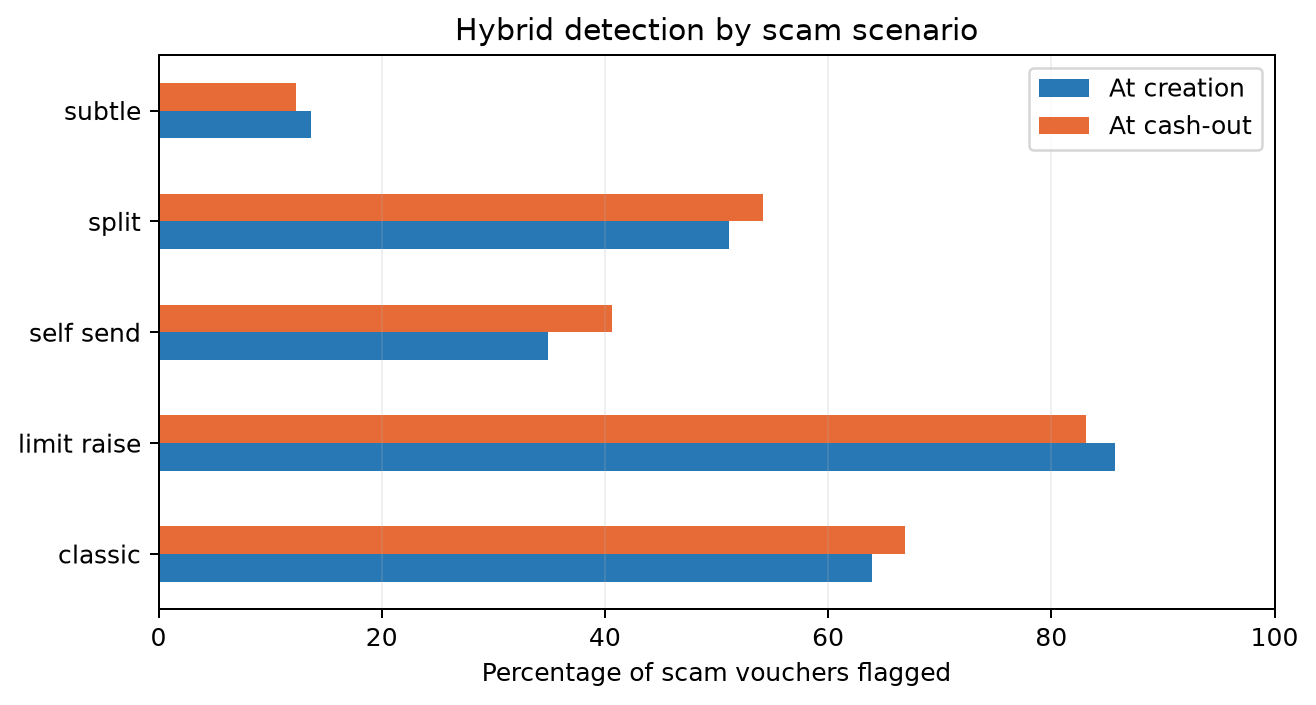
\includegraphics[width=.92\linewidth]{discussion_figures/scenario_recall.png}
\caption{Percentage of scam vouchers flagged by the hybrid in each scenario.}
\end{figure}

\begin{table}[htbp]
\centering\small
\caption{Hybrid alert rates by scenario. For scam rows, the rate is recall; for legitimate rows, it is the false-alarm rate within that scenario. Counts show flagged vouchers / total vouchers, rather than distinct scam episodes.}
\begin{tabularx}{\linewidth}{Yrrrr}
\toprule
\textbf{Scenario} & \textbf{Creation} & \textbf{Rate (\%)} & \textbf{Cash-out} & \textbf{Rate (\%)} \\
\midrule
Classic scam & 172 / 269 & 63.9 & 180 / 269 & 66.9 \\
Limit-raise scam & 162 / 189 & 85.7 & 157 / 189 & 83.1 \\
Self-send scam & 67 / 192 & 34.9 & 78 / 192 & 40.6 \\
Split-voucher scam & 183 / 358 & 51.1 & 194 / 358 & 54.2 \\
Subtle scam & 21 / 154 & 13.6 & 19 / 154 & 12.3 \\
Legitimate emergency & 176 / 268 & 65.7 & 141 / 264 & 53.4 \\
Legitimate new-phone use & 100 / 550 & 18.2 & 38 / 531 & 7.2 \\
Legitimate travel & 2 / 288 & 0.7 & 2 / 282 & 0.7 \\
\bottomrule
\end{tabularx}
\end{table}

The legitimate scenarios showed the other side of this difficulty. Emergency payments deliberately shared behaviours such as unusual amounts and recent account changes with scams, and the hybrid flagged 65.7\% of these vouchers at creation and 53.4\% at cash-out. By comparison, ordinary legitimate vouchers had false-alarm rates of 0.73\% and 0.42\%. The low overall false positive rate therefore concealed a much greater burden for customers making legitimate emergency payments. This overlap was central to the problem being investigated: a suspicious pattern could justify closer review without revealing whether the customer had a valid reason for the payment.

\FloatBarrier\subsection{Prototype demonstration}

The dashboard connected these detection results to the information someone reviewing an alert could inspect. Its queue ranked vouchers by the saved hybrid score and displayed amounts, risk bands and triggered rule indicators. From an alert, the customer history view allowed the voucher to be considered alongside earlier scored vouchers and recent account events. The model comparison view then showed the results over the complete test period, providing context for the method used to generate the alerts.

The interface reused the same hybrid scores and alert thresholds as the evaluation, with High and Critical bands corresponding to an alert. Users could select the scoring stage and date, while an optional ground-truth view supported inspection of the simulated outcomes. The displayed rule indicators explained which checklist conditions were present, rather than the internal One-Class SVM decision. The demonstration consequently showed how scores and surrounding information could support review; because it replayed precomputed results, it did not establish live processing speed or the effectiveness of analyst decisions.

\FloatBarrier\subsection{Interpretation and limitations}

The findings address the main research question by showing that behavioural risk scoring identified a share of the simulated scam-associated vouchers at both creation and cash-out. The hybrid had the highest test F1 among the five approaches, but still missed almost half of the scams. Its stronger results on prominent warning patterns and weaker results on subtle scams show the limits of the detection demonstrated here. Behavioural scoring supplied a basis for raising suspicion, while the results did not support treating every alert as confirmed fraud.

For the question of relevant indicators, the EDA showed differences in amounts, recent limit changes and redemption timing, together with overlap in legitimate behaviour. These observations help explain why combinations of indicators were considered in the prototype. They do not establish a ranking of feature importance, because the evaluation did not measure the effect of removing individual features. For the comparison of scoring approaches, the hybrid offered the better F1 at both stages, while rules remained more precise. Its value therefore lay in detecting more scams while accepting more false alerts, rather than improving every measure at once.

This trade-off also informs the question of intervention. The high false-alarm rate on legitimate emergencies supports considering additional verification or analyst review before a decision to block a voucher. The queue and customer history views demonstrated how information could be presented for that purpose. However, the study did not test customer responses, the effect of a warning or delay, or financial losses prevented, so the effectiveness of those interventions remains unmeasured.

These conclusions must also be considered within the limits of the dataset. Customer behaviour, scam probabilities and rule weights were simulation assumptions, and passing the consistency checks did not establish that the records represented a real bank's customers. Labels were excluded from anomaly fitting but used for validation selection and during dataset development, and the data had already been examined. In addition, the scoring stages differed in eligible records as well as available information. The results therefore provide evidence for the comparison in this controlled simulation, while further work with independently collected banking data would be needed to assess its practical performance.

\FloatBarrier\section*{References}

Le Borgne, Y.-A., Siblini, W., Lebichot, B. and Bontempi, G. (2022). \emph{Reproducible Machine Learning for Credit Card Fraud Detection — Practical Handbook}. Université Libre de Bruxelles. \href{https://fraud-detection-handbook.github.io/fraud-detection-handbook/Chapter\_4\_PerformanceMetrics/ThresholdBased.html}{Threshold-based metrics}.

% END DISCUSSION BODY
\end{document}
